% !TeX spellcheck = fr_FR
\chapter{Chapitre 2 : Bcrypt sur FPGA}

Tout le travail, dont je vais parler dans ce chapitre a été fait en grande partie durant le projet de semestre.
Comme expliqué dans le chapitre précèdent, pour le bcrypt, je suis reparti d'une implémentation déjà existante en \gls{vhdl}.

\section{Bcrypt sur FPGA}

Après lecture du code source, j'ai pu déduire l'architecture suivante :

\begin{figure}[tbph!]
	\centering
	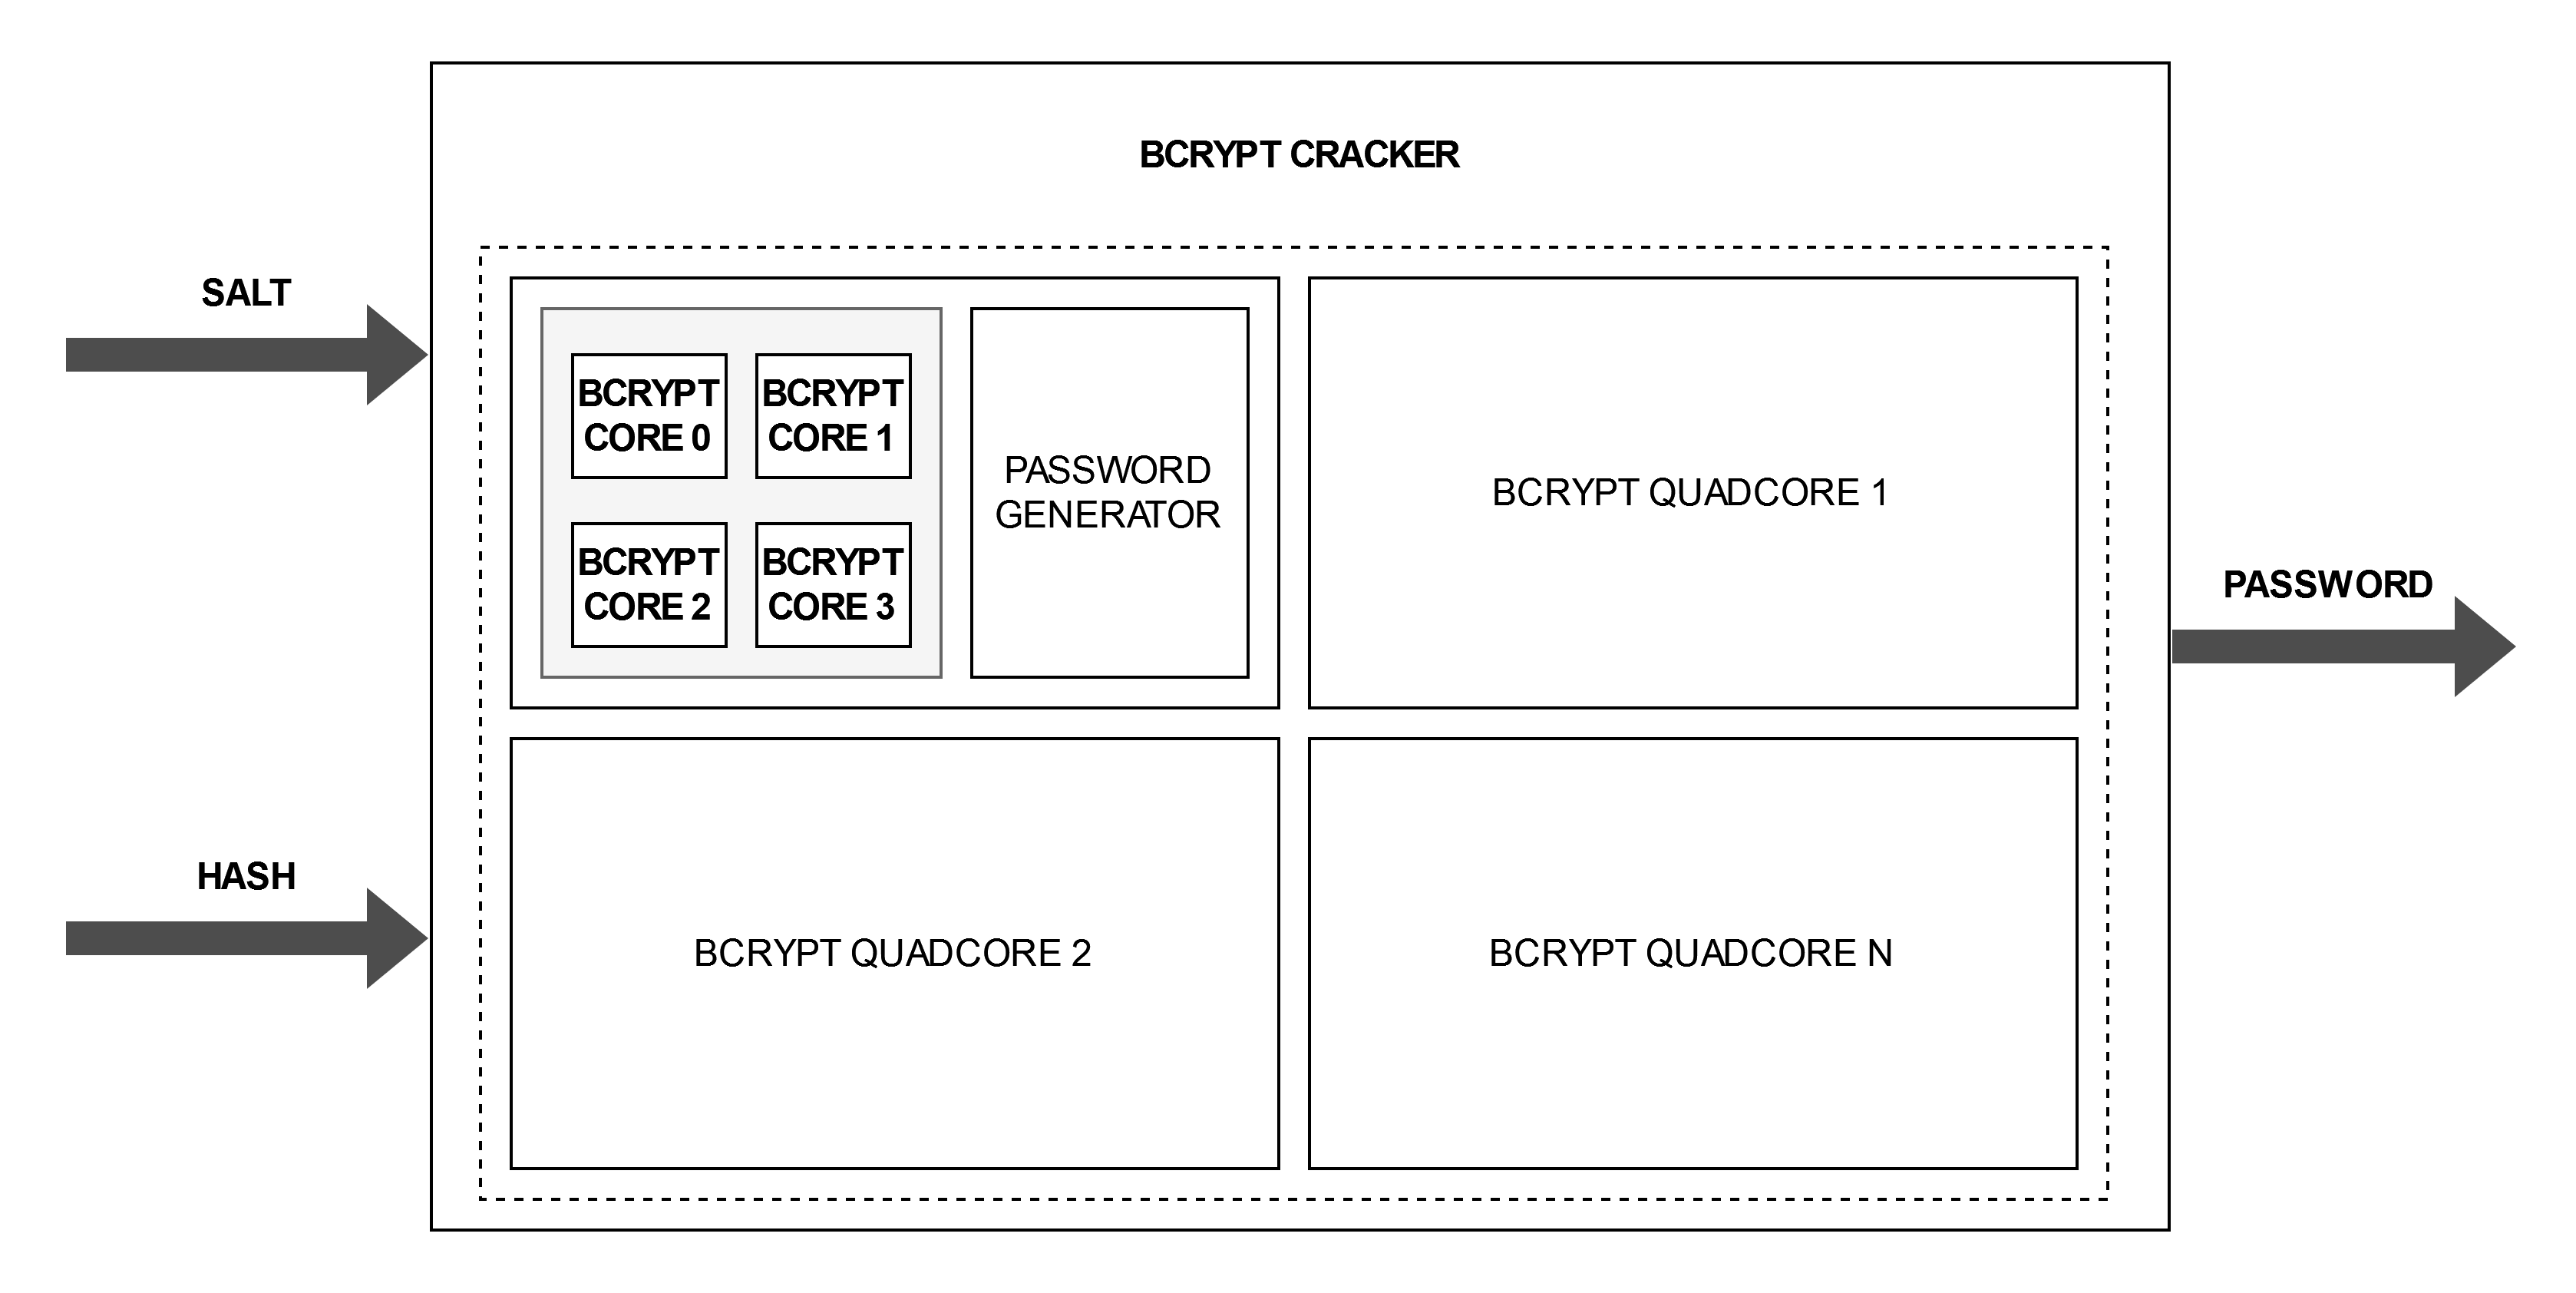
\includegraphics[width=0.9\linewidth]{bcrypt_architecture}
	\caption[Architecture Bcrypt sur FPGA]{Architecture Bcrypt sur FPGA. Source : réalisé par Kandiah Abivarman}
	\label{fig:bcrypt_architecture}
\end{figure}

L'architecture contient 4 modules clé, il y a d'abord le bcrypt core qui est le cœur de calcul qui va s'occuper de faire la fonction de hachage bcrypt. 
Ensuite, le password generator qui va s'occuper de générer les différents mots de passe pour l'attaque par bruteforce. 
Puis, le bcrypt quadcore qui va s'occuper d'instancier quatre bcrypt core et un générateur de mots de passe pour alimenter les cœurs en mot de passe. 
Enfin, le bcrypt cracker va instancier le nombre souhaité de quadcore, s'occuper de la gestion des différents coeurs et retransmettre le mot de passe lorsque il est retrouvé.

\subsection{Bcrypt Core}

Le bcrypt core était la partie qui m'intéressait le plus dans ce code source, car c'est le module qui s'occupe de faire le hachage et c'était ce que je cherchais initialement parmi les implémentations déjà existantes.

J'ai donc entamé le projet en testant le module avec de la simulation en utilisant le testbench fourni, mais je me suis vite rendu compte que le testbench fourni ne fonctionnait pas. 
En effet, le testbench fourni semble avoir été fait pour une ancienne version du bcrypt core avec une interface totalement différente, rendant le fichier de test obsolète.

Afin de pouvoir implémenter moi-même le testbench de ce module, je suis passé par une première phase ou j'ai analysé le code afin de comprendre l'interface du bcrypt core.

J'ai pu notamment identifier les \gls{i/o} qui permettant le contrôle du module, les \gls{i/o} de la fonction de hachage (mot de passe, salt et hash) et les \gls{i/o} qui vont permettre l'initialisation de la mémoire pour les clés de chiffrement. 
Le cost de la fonction de hachage est lui fixé par une constante situé dans un fichier à part regroupant d'autres constantes du système.

\begin{figure}[tbph!]
	\centering
	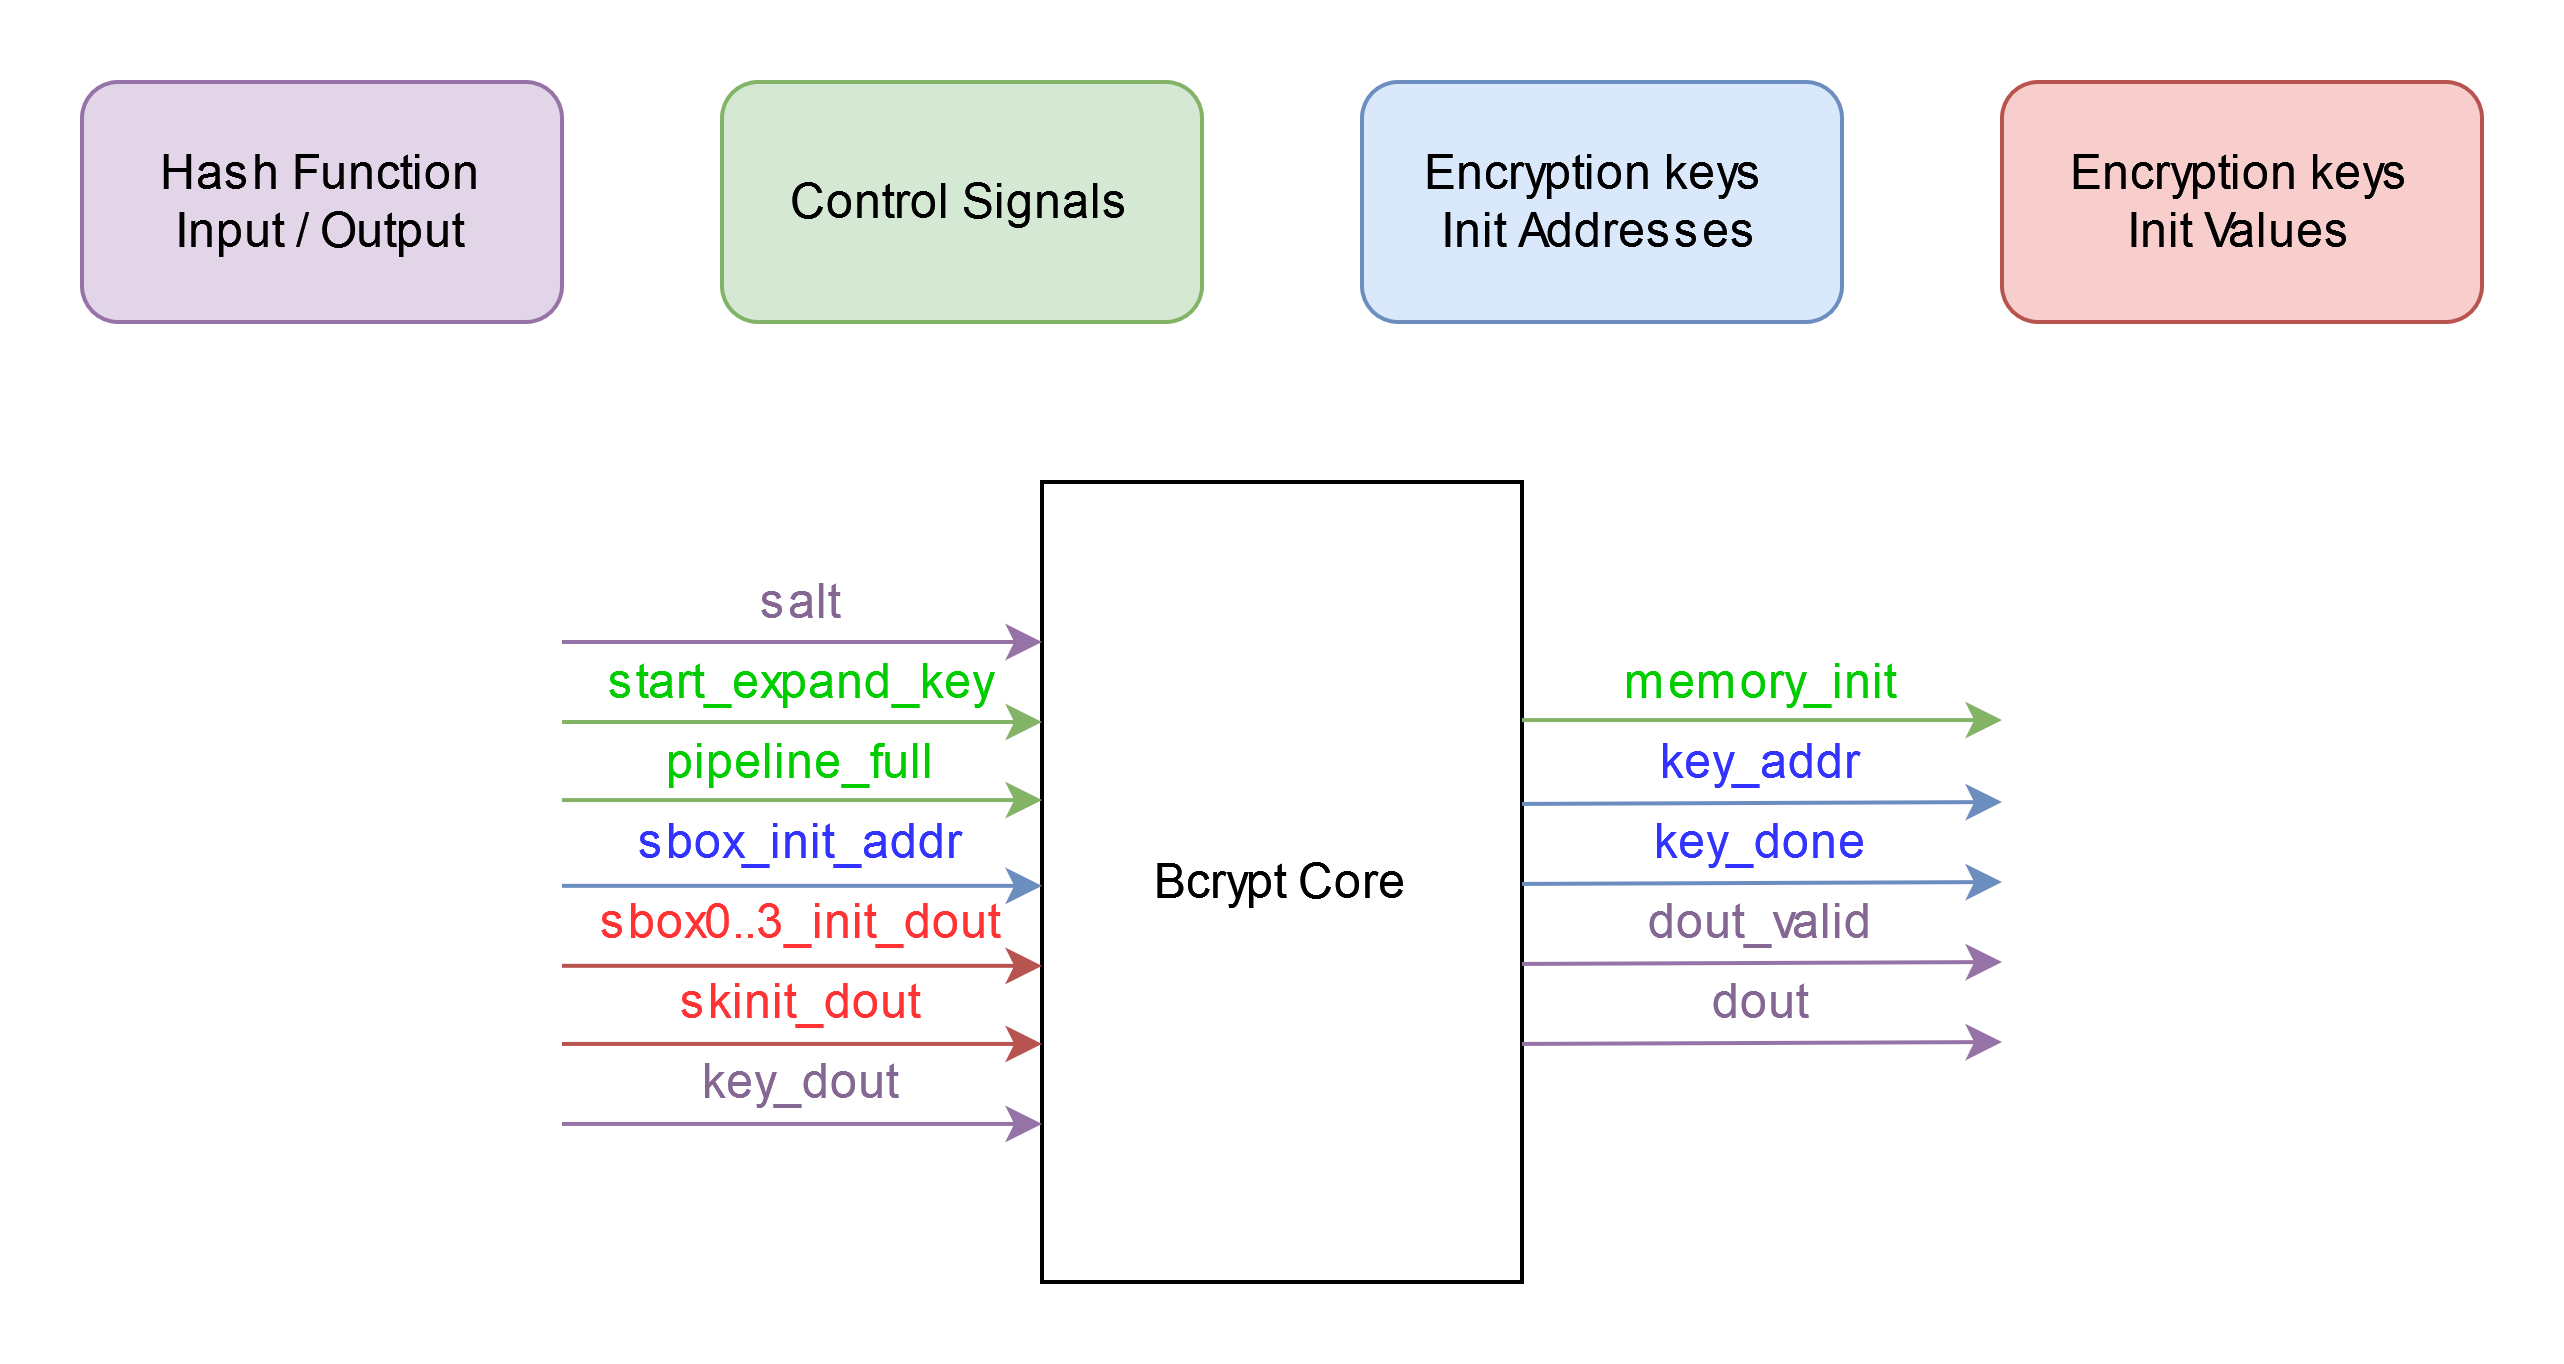
\includegraphics[width=0.9\linewidth]{bcrypt_core_interface}
	\caption[Interface du Bcrypt core]{Interface du Bcrypt core. Source : réalisé par Kandiah Abivarman}
	\label{fig:bcrypt_core_interface}
\end{figure}


Après une identification des \gls{i/o}, j'ai examiné les différents processus et instanciations qui ont lieu dans le module bcrypt core. 
Il y a tout d'abord plusieurs \gls{bram} qui sont utilisés pour le stockage des clés de chiffrement, un module qui s'occupe du chiffrement blowfish, une machine d'état pour gérer les différentes étapes de la fonction de hachage et différents compteurs nécessaires à l'adressage mémoire et à la machine d'état.

\newpage

\begin{figure}[tbph!]
	\centering
	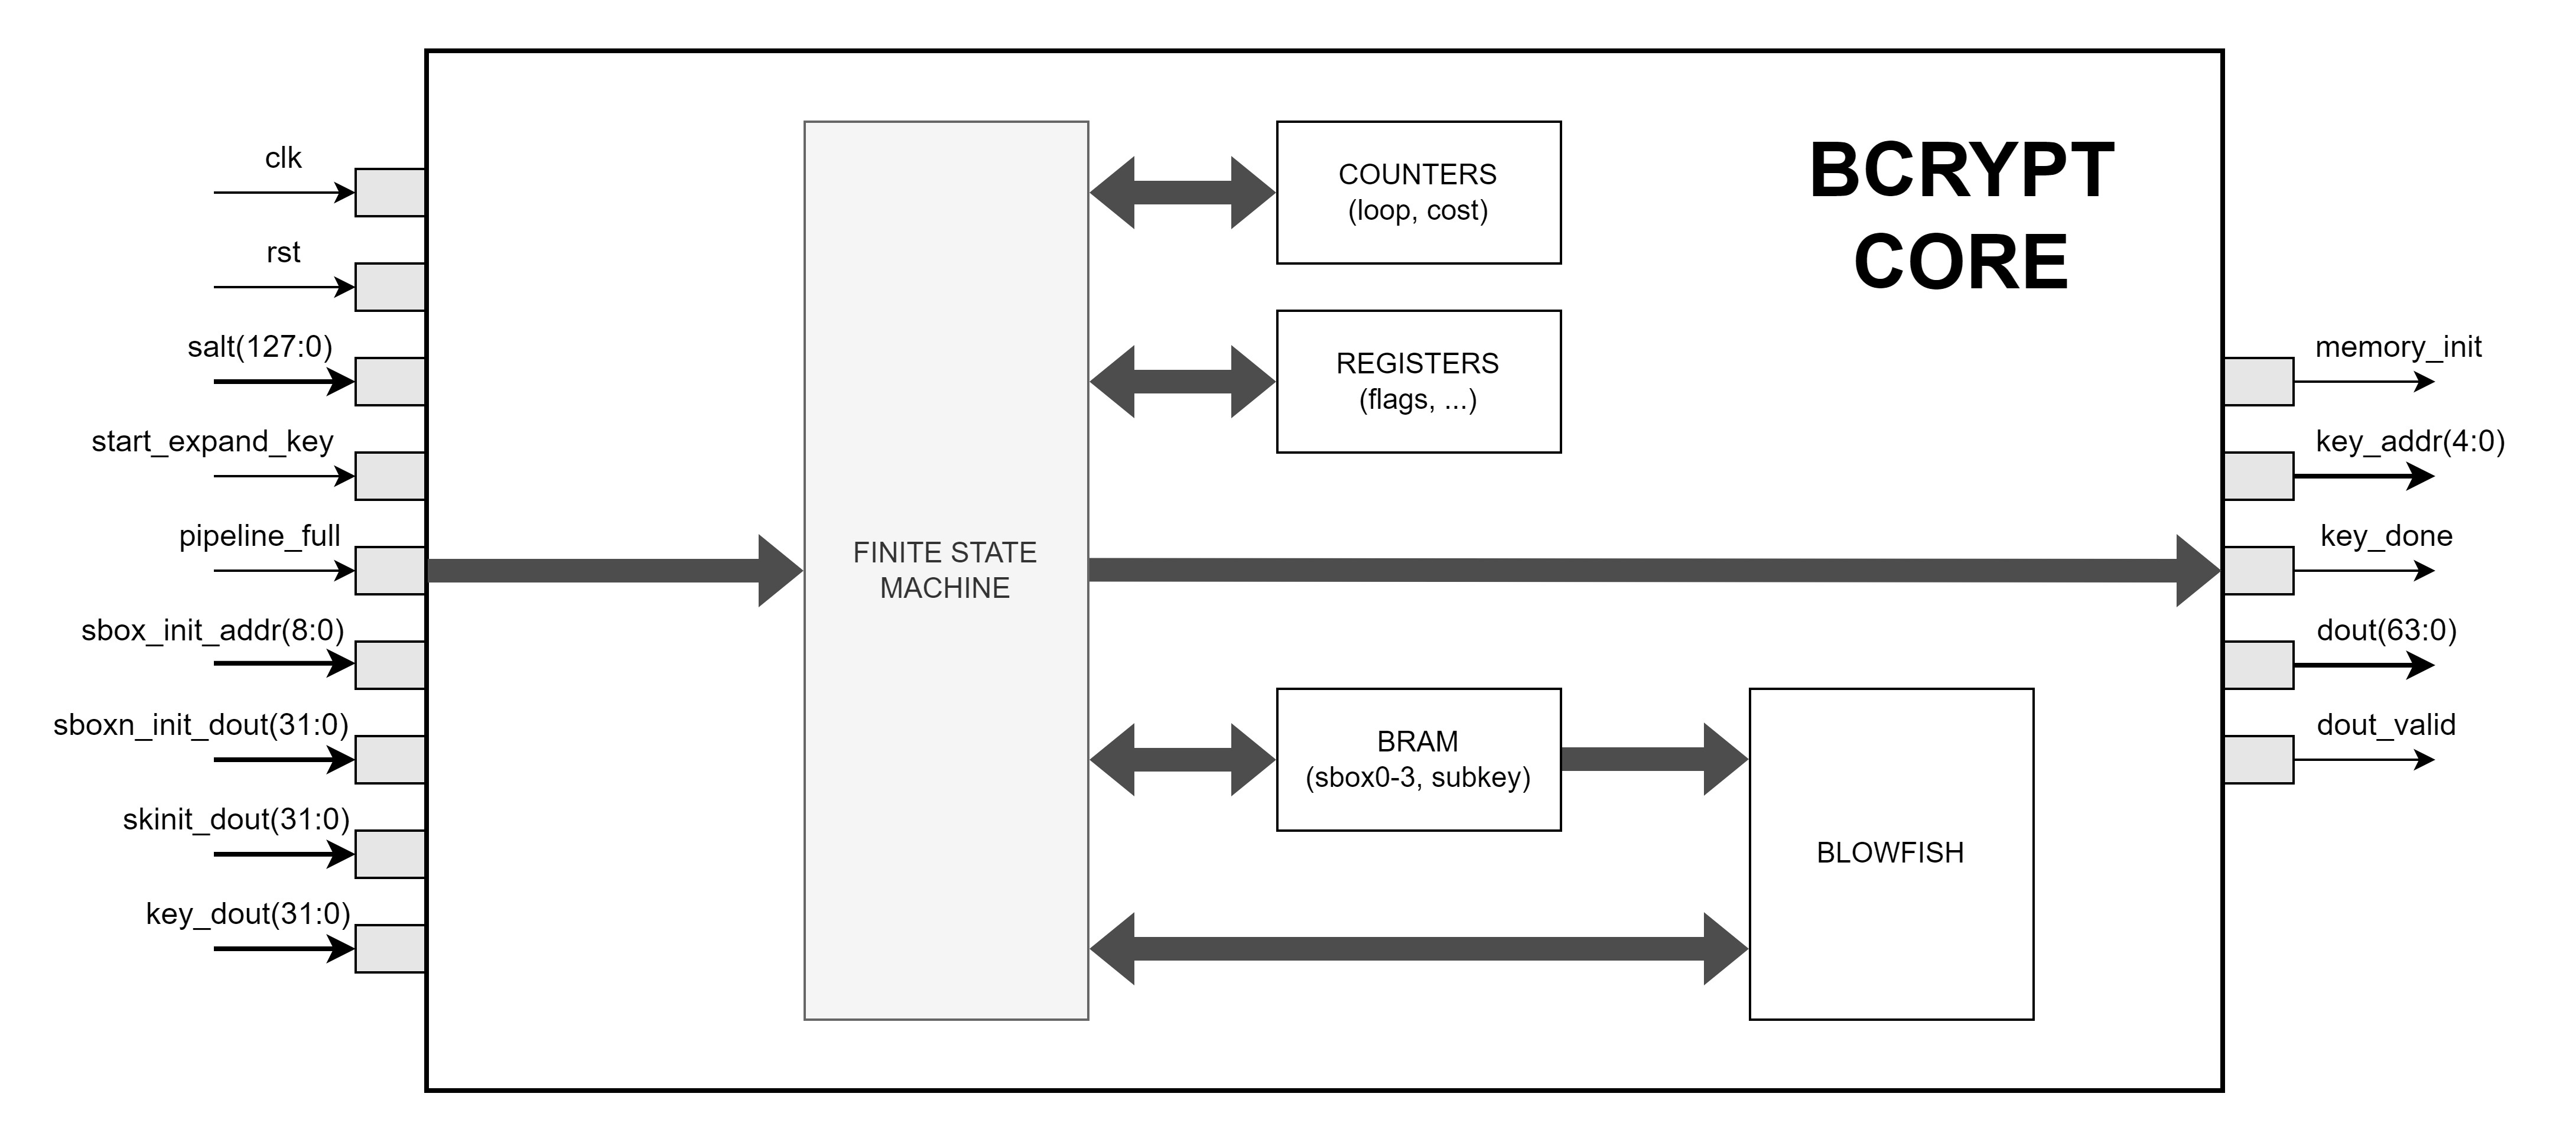
\includegraphics[width=0.9\linewidth]{bcrypt_core_simplified}
	\caption[Schéma Bcrypt core simplifié]{Schéma du Bcrypt core simplifié. Source : réalisé par Kandiah Abivarman}
	\label{fig:bcrypt_core_simplified}
\end{figure}

La machine d'état contient 18 états, mais je vais la simplifier pour l'explication. 
Tout d'abord, le module va attendre un signal du module parent afin de démarrer, après réception du signal, la phase d'initialisation de la mémoire est lancée. 
Cette étape consiste à initialiser les clés de chiffrement, pour se faire, il faut fournir au module l'adresse mémoire où l'on souhaite écrire dans les \gls{bram} et les données que l'on souhaite écrire dans notre cas les différents décimaux de PI. 
Après la phase d'initialisation de mémoire, le module va de nouveau attendre un signal en entrée afin de procéder au calcul des clés de chiffrement. 
Cette étape consiste en 7 états dans la machine d'état et va reboucler un certain nombre de fois en fonction du cost. Après les calculs des clés de chiffrement, vient le chiffrement du mot magique qui va nous donner notre hash. 
Le port de sortie pour le hash fait une taille de 64 bits, mais un hash fait 192 bits, de ce fait le module ressort le hash en trois morceaux. 
Le processus de chiffrement est donc séparé en trois étapes pour chaque morceau du hash, chaque étape consiste en réalité à 2 états, un premier état de préparation et ensuite un état de calcul.

\newpage

\begin{figure}[tbph!]
	\centering
	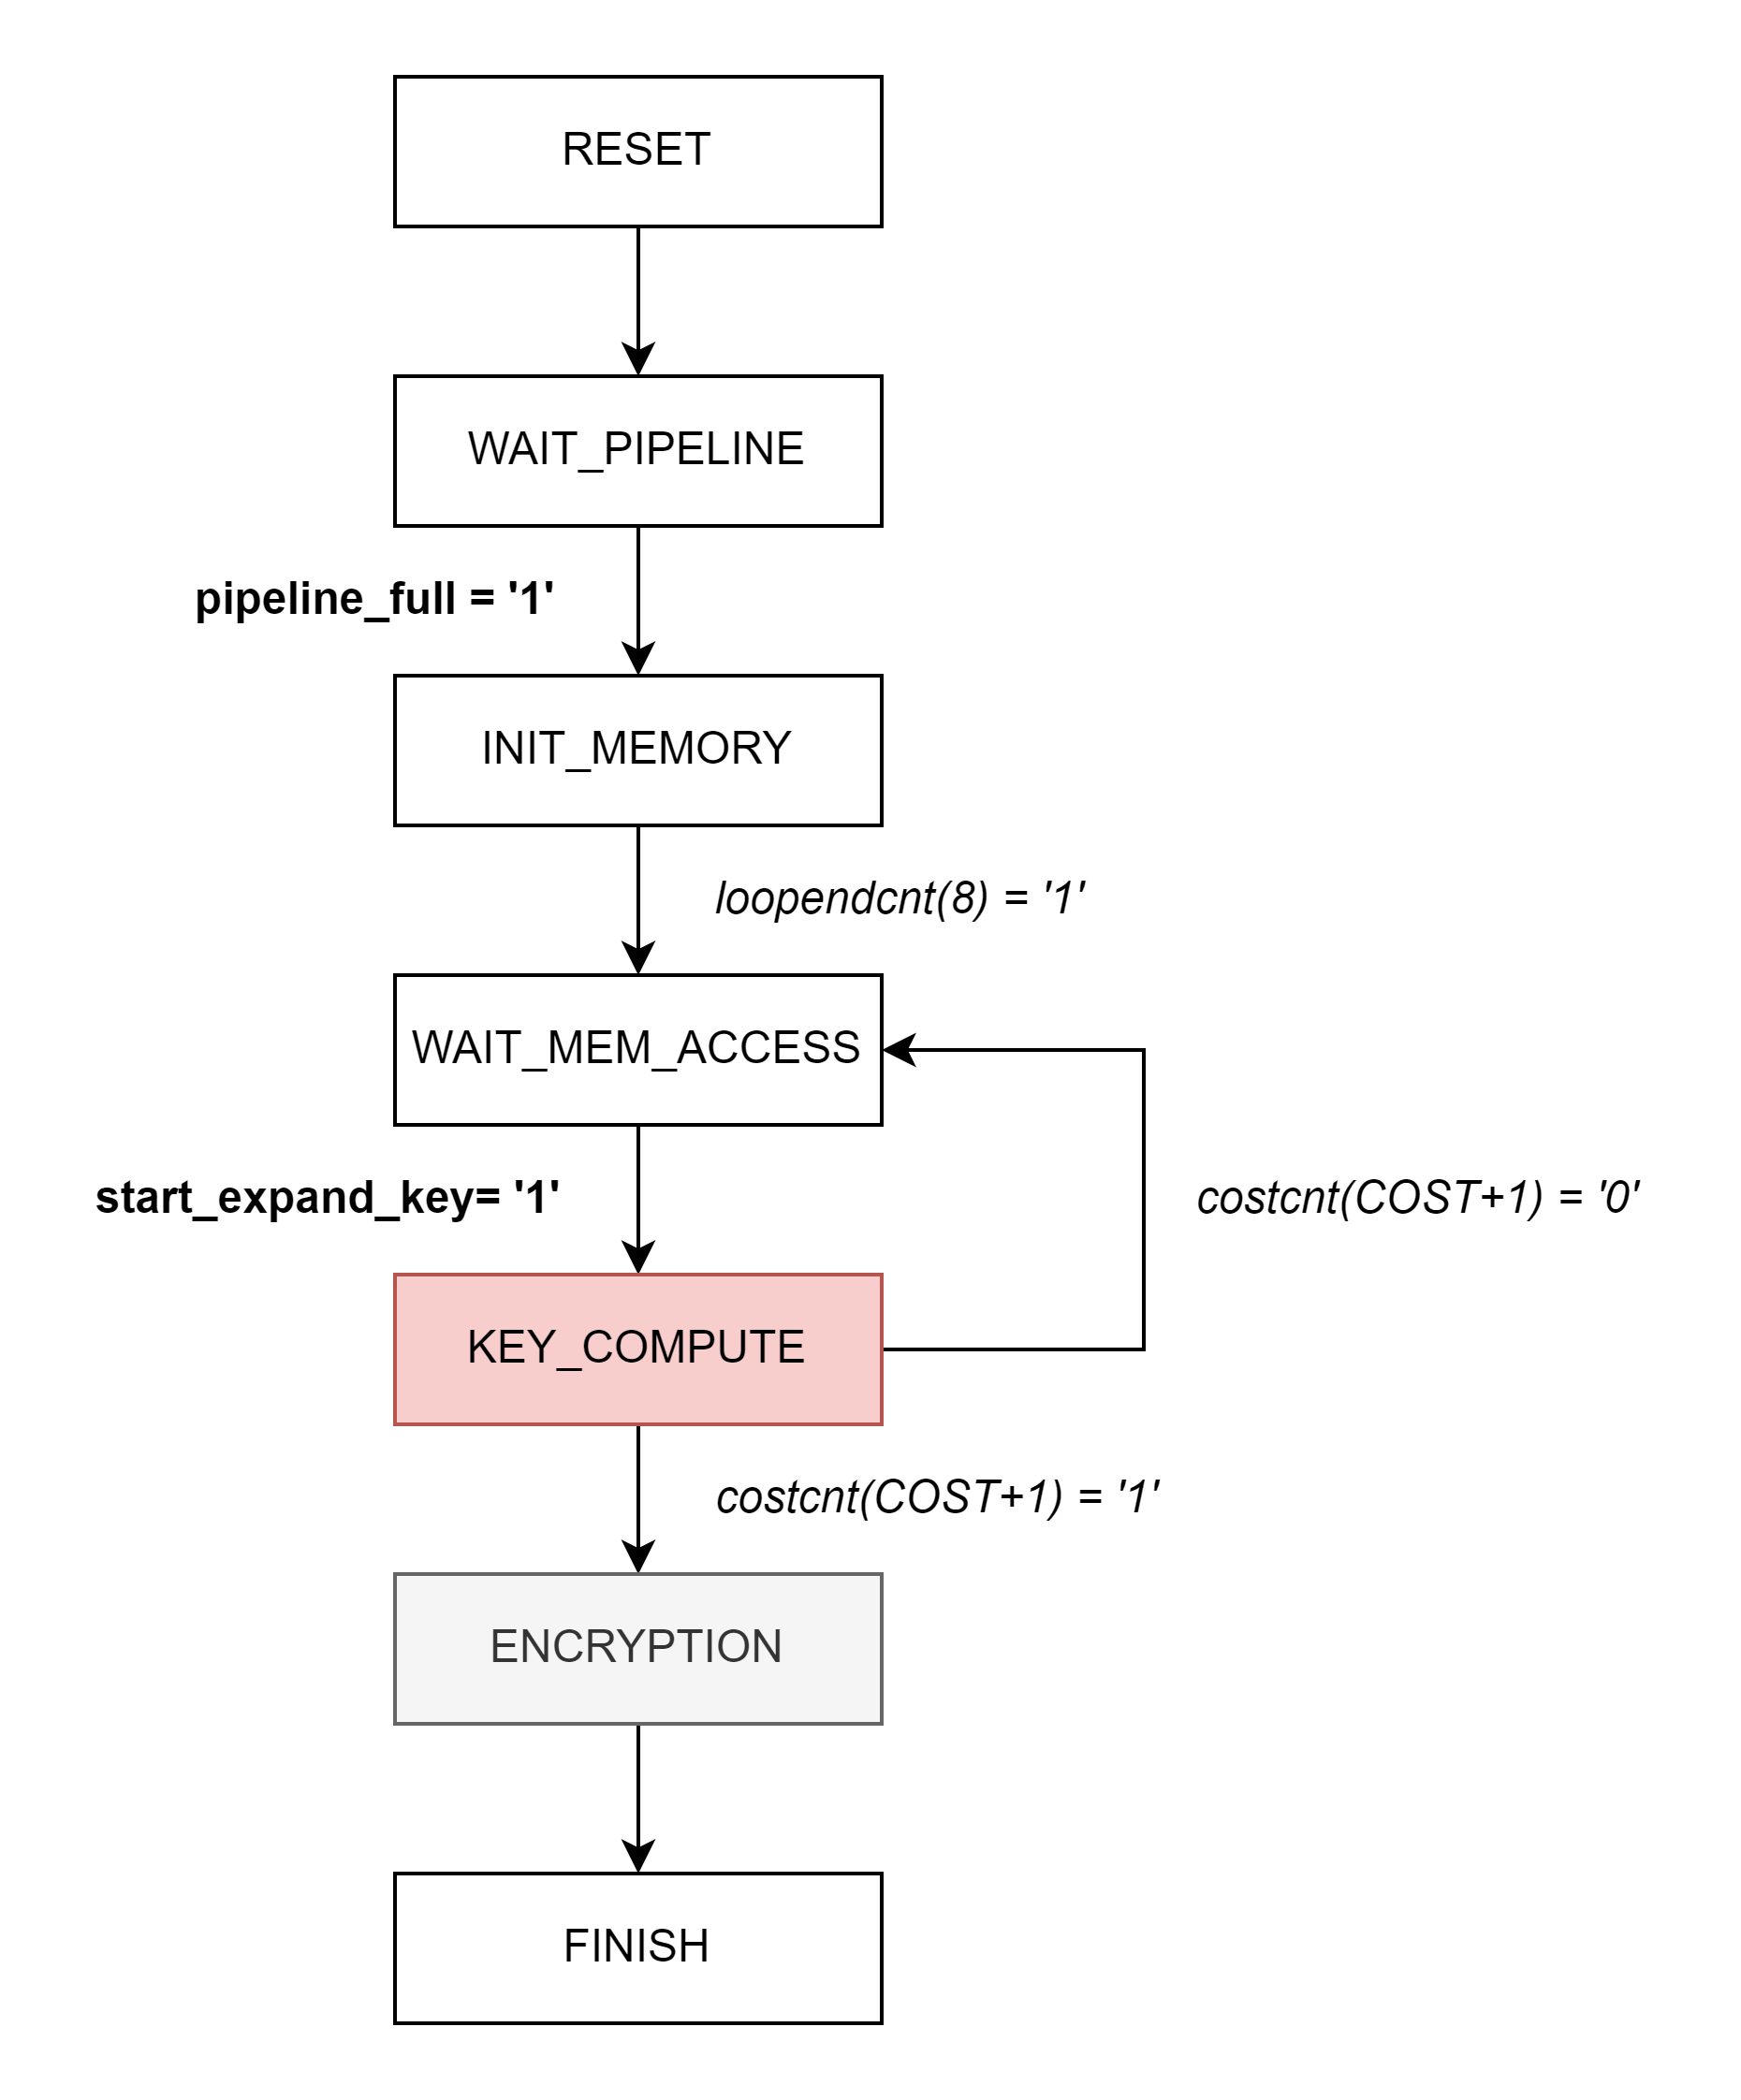
\includegraphics[width=0.7\linewidth]{bcrypt_core_simplified_fsm}
	\caption[Machine d'état Bcrypt core simplifié]{Machine d'état du Bcrypt core simplifié. Source : réalisé par Kandiah Abivarman}
	\label{fig:bcrypt_core_simplified_fsm}
\end{figure}

Par la suite, j'ai fait des simulations en testant des valeurs dans les différentes entrées afin d'essayer de comprendre les timings attendus par le module. 
Après ces analyses, j'ai pu comprendre ce que le module attendait en entrée et les différents timings attendus.

\newpage

\begin{figure}[tbph!]
	\centering
	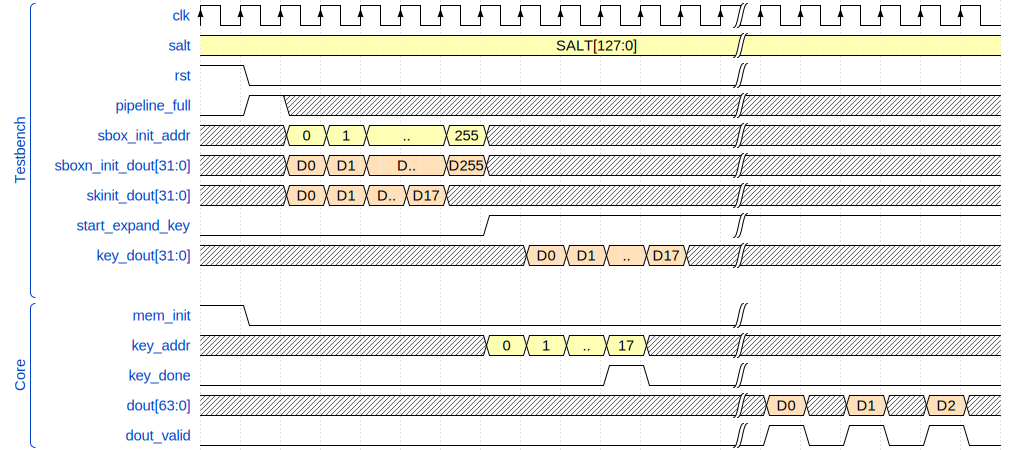
\includegraphics[width=0.9\linewidth]{bcrypt_tb_timing}
	\caption[Timing du bcrypt]{Timing du bcrypt. Source : réalisé par Kandiah Abivarman}
	\label{fig:bcrypt_tb_timing}
\end{figure}

Le port \textit{pipeline\_full} va permettre de démarrer l'initialisation de la mémoire dans le module. 
Lors de l'initialisation de la mémoire, il faut fournir au module les adresses mémoires où l'on souhaite écrire avec \textit{sbox\_init\_addr} et on va fournir les valeurs initiales des \gls{sbox} sur \textit{sboxn\_init\_dout} et des subkeys sur \textit{skinit\_dout}. 
Suite à cela, on va utiliser le port \textit{start\_expand\_key} afin de démarrer le calcul des clés de chiffrement. 
Pour le calcul des clés, on va donner à \textit{key\_dout} la bonne partie du mot de passe en fonction de l'adresse mémoire fourni par \textit{key\_addr}, puis le port \textit{key\_done} va signaler la fin des calculs des clés. 
Pour finir, les différents morceaux du hash sont données par \textit{dout} et le port \textit{dout\_valid} va avertir lorsque les différents morceaux sont prêts.

Après analyses des différents timings attendus, j'ai pu refaire le testbench du module bcrypt core est valider son bon fonctionnement.

\newpage

\subsection{Password Generator}

Le password generator à un rôle assez important, car c'est le module qui va s'occuper de générer les différents de mots de passe à tester pour l'attaque.

J'ai donc repris la même démarche que pour le module précèdent afin de comprendre le fonctionnement du bloc. 
C'est à partir de ce module que j'ai commencé à rencontrer des difficultés notamment dû à des constantes qui ont été fixées avec des valeurs sans aucun sens et sans explications. 
Après quelque temps passé avec le simulateur, j'ai réussi à comprendre le comment marche le module et comment utiliser les constantes et les fixer pour avoir le fonctionnement souhaité. 

Dans ce module, les mots de passe sont générés à l'aide de compteur, il y a un compteur par caractère que l'on souhaite générer pour le mot de passe. 
Chaque valeur de compteur va être convertie en valeur ASCII afin de retrouver les caractères que l'on utilise dans nos mots de passe. 
La conversion est assez simple, nous avons dans l'ordre l'alphabet en minuscule, l'alphabet en majuscule et les chiffres. 

\begin{figure}[tbph!]
	\centering
	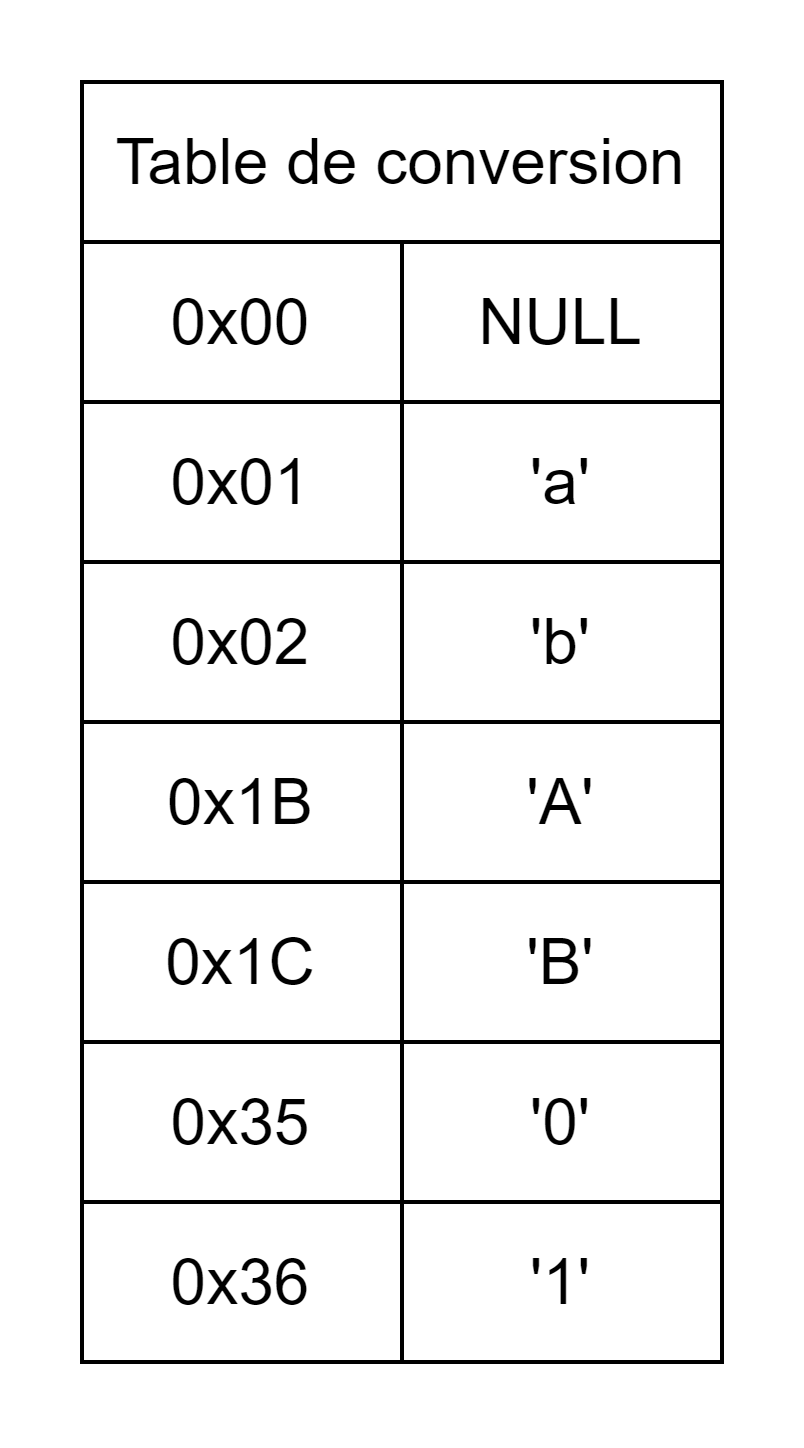
\includegraphics[width=0.25\linewidth]{conversion_table}
	\caption[Table de conversion]{Table de conversion. Source : réalisé par Kandiah Abivarman}
	\label{fig:conversion_table}
\end{figure}

Enfin, les différents caractères générés sont concaténés afin d'avoir au final un mot de passe. 
La fonction de hachage Bcrypt a besoin en entrée un mot de passe de 72 bytes, donc lorsque un mot de passe plus petit est utilisé, on va répéter en boucle le mot de passe en boucle jusqu'à atteindre les 72 bytes. 
Il est aussi nécessaire de délimiter chaque répétition par un caractère null. 
Ce module prend en compte ce détail est va s'occuper de remplir les 72 bytes comme il se doit lorsque le mot de passe généré est plus petit.

Un point à retenir est que lorsque l'on instancie le module, on peut définir le compteur initial et la taille du mot de passe initial. 
Par exemple, si on initialise le compteur à zéro et la taille du mot de passe à un, nous aurons comme premier mot de passe le caractère 'a' puis 'b' et ainsi de suite. 
Donc, lors de l'instanciation, il est nécessaire d'initialiser les compteurs intelligemment afin d'avoir l'attaque la plus optimale.

\subsection{Bcrypt Quadcore}

Le bcrypt quadcore est le bloc qui va s'occuper d'instancier les deux modules dont j'ai parlé précédemment, c'est aussi dans ce module que j'ai rencontré de nombreux erreurs que j'ai dû corriger afin d'avoir un programme fonctionnel.

Ce module contient le générateur de mot de passe, une \gls{bram} pour stocker les mots de passe généré, quatre bcrypt core, une machine d'état et des compteurs.

Le système va tout d'abord avoir un premier état d'initialisation dans laquelle quatre mots de passe vont être générés pour chaque bcrypt core. 
Après la génération, chaque bcrypt core va calculer le hash en fonction de son mot de passe. 
Lorsque les calculs sont finis, les hash vont être comparé à l'hash que l'on souhaite casser, lorsque un hash correspond, le module va ressortir le mot de passe correspondant.
Toutefois, si les hash ne correspondent pas, alors le système va retourner au premier état d'initialisation. 
Enfin, après un certain nombre d'essais fixé lors de l'instanciation du module, le système s'arrête.

\newpage

\begin{figure}[tbph!]
	\centering
	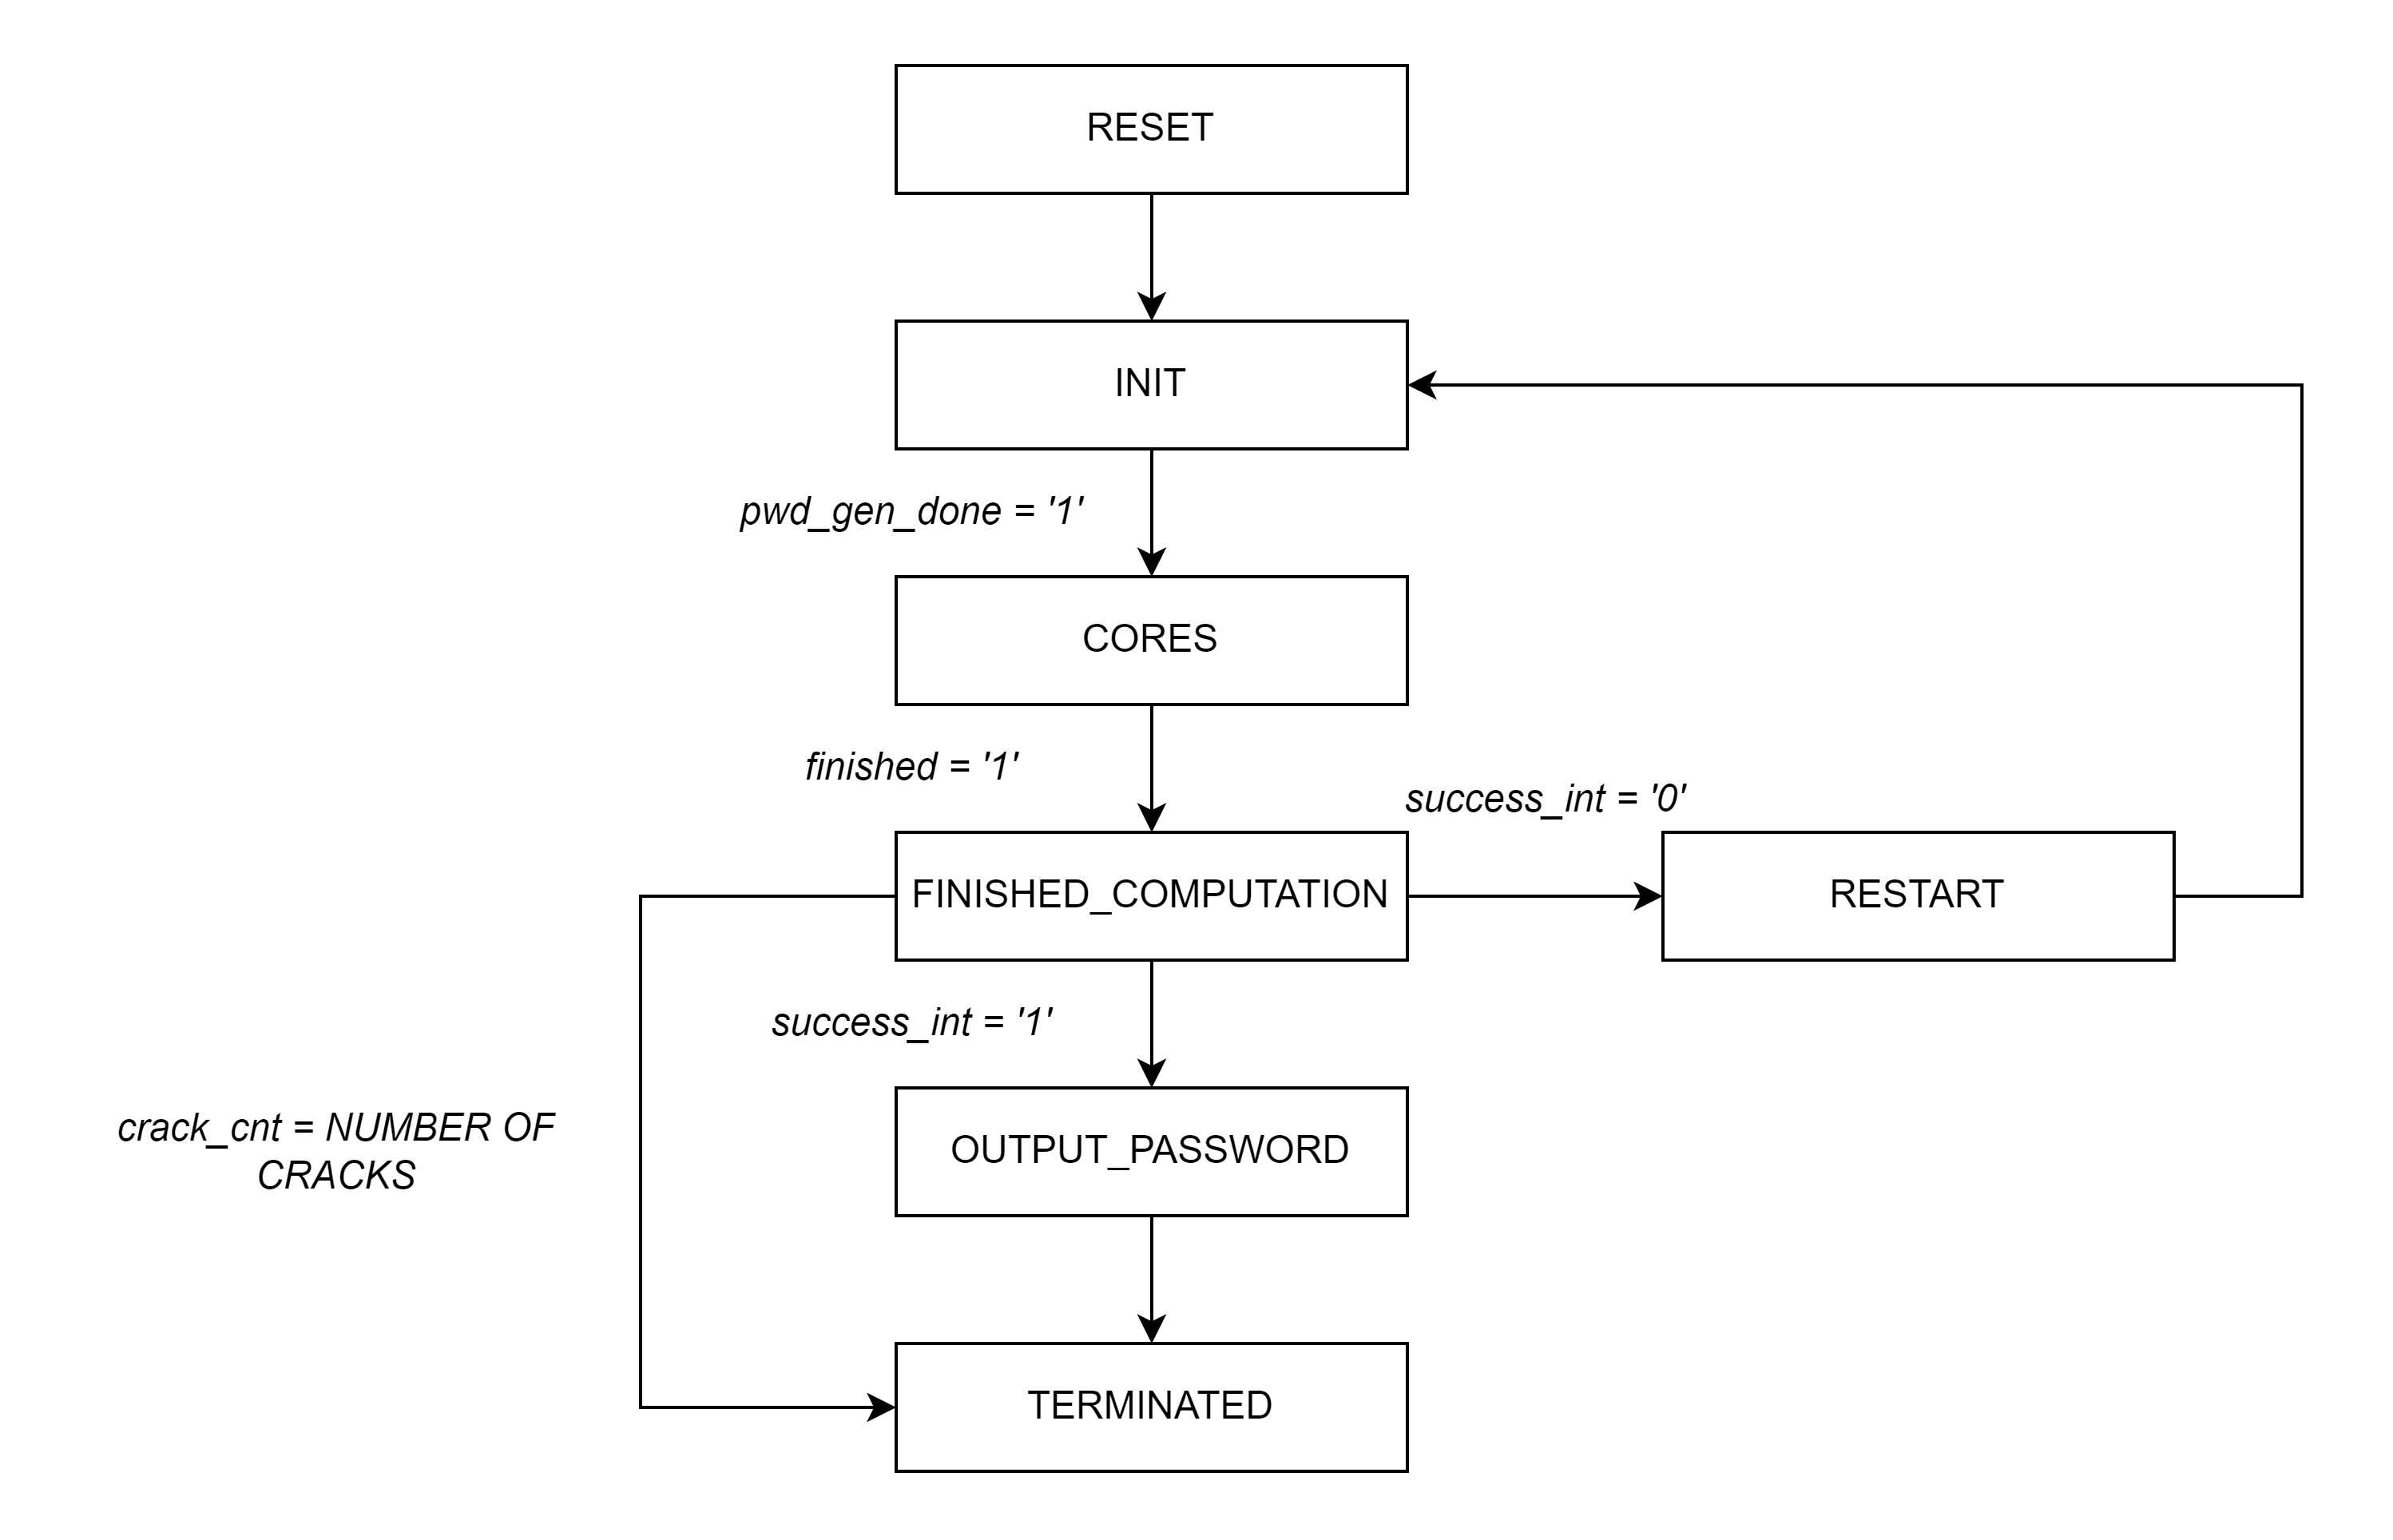
\includegraphics[width=0.7\linewidth]{bcrypt_quad_simplified_fsm}
	\caption[Machine d'état Bcrypt quadcore simplifié]{Machine d'état du Bcrypt quadcore simplifié. Source : réalisé par Kandiah Abivarman}
	\label{fig:bcrypt_quad_simplified_fsm}
\end{figure}

\subsection{Bcrypt Cracker}

Ce module va s'occuper d'instancier deux \gls{bram} contenant l'état initial des clés de chiffrement qui vont, elles même permettre d'initialiser les \gls{bram} présentes dans les bcrypt core. 
C'est aussi dans le bcrypt cracker qu'il y a l'instanciation des quadcore, le nombre souhaité de quadcore et le nombre d'essais est réglable dans le code.

Ce module est au final la partie qui va s'occuper du craquage de mot de passe, elle va prendre en entrée le salt et le hash du mot de passe que l'on souhaite retrouver et va ressortir le mot de passe lorsque il est retrouvé.  

Afin de bien vérifier le fonctionnement de ce module et du bcrypt quadcore, j'ai utilisé le testbench fourni et j'ai ajouté la vérification de la sortie qui manquait au fichier de test.

Pour ce faire, j'ai regardé au niveau de la simulation afin d'étudier le comportement des sorties du module en fonction des entrées.

Le module à deux entrées qui sont le salt et le hash que l'on souhaite casser et quatre ports de sortie.
Il y a d'abord le port \textit{done} qui va permettre d'avertir lorsque le système est dans son état final, c'est-à-dire lorsque il a trouvé le mot de passe ou qu'il a atteint le nombre d'essais maximaux.
Ensuite, il y a \textit{success} qui est mis à un lorsque le mot de passe est trouvé.
Puis, il y a \textit{dout} qui va nous fournir le mot de passe lorsque il est trouvé et \textit{dout\_we} qui est un signal de permission si l'on souhaite écrire le mot de passe dans une mémoire par exemple.

\newpage

\begin{figure}[tbph!]
	\centering
	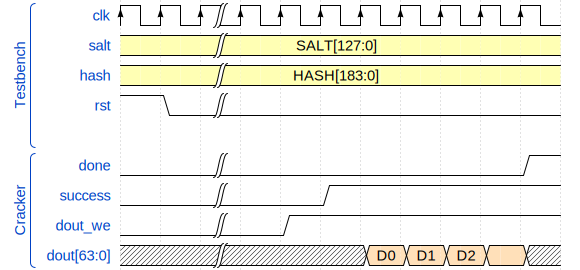
\includegraphics[width=0.9\linewidth]{bcrypt_cracker_tb_timing}
	\caption[Timing du bcrypt cracker]{Timing du bcrypt cracker. Source : réalisé par Kandiah Abivarman}
	\label{fig:bcrypt_cracker_tb_timing}
\end{figure}

Initialement, lors de mes premiers tests, le système semblait fonctionnel. Pour tester le système, je mettais des hash de mot de passe assez simple a casser comme 'a' ou 'b'.
J'ai initialisé le compteur du générateur de mot de passe à 0, de ce fait les premiers mots de passe que le module va essayer sont justement 'a', 'b', 'c' et 'd'.

Toutefois, lorsque j'ai testé avec un mot de passe tel que 'z' qui va obliger plusieurs essais au système avant de trouver, le système s'arrête après le premier essai.
Le système avait considéré avoir trouvé le mot de passe alors que ce n'était pas le cas. J'ai pu régler ce cas, après avoir identifié une condition incorrecte dans le quadcore.
Par la suite d'autres problèmes sont apparus, par exemple des problèmes de réinitialisation de compteur lorsque le système va essayer des nouveaux mots de passe.
Tous les problèmes à ce niveau-là provenaient du bcrypt quadcore et ont pu être corrigé grâce à la simulation.
